\section{hoodie}
Hoodie ist eine JavaScript Bibliothek für offlinefähige Webapplikationen, die ein komplettes Backend zur Verfügung stellt. Wird Hoodie für die Entwicklung einer Webanwendung verwendet, muss also lediglich das Frontend implementiert werden. Den Rest erledigt die Bibliothek. Über eine integrierte Programmierschnittstelle kommuniziert die Anwendung mit dem von Hoodie zur Verfügung gestelltem Backend. Über das \gls{API} können unter Anderen BenutzerInnen authentifiziert, Daten gespeichert und synchronisiert werden~\cite{hoodie}.\\
Anhand der Abbildung \ref{fig:hoodie} wird erklärt wie Hoodie funktioniert.
\begin{figure}[H]
  \centering
  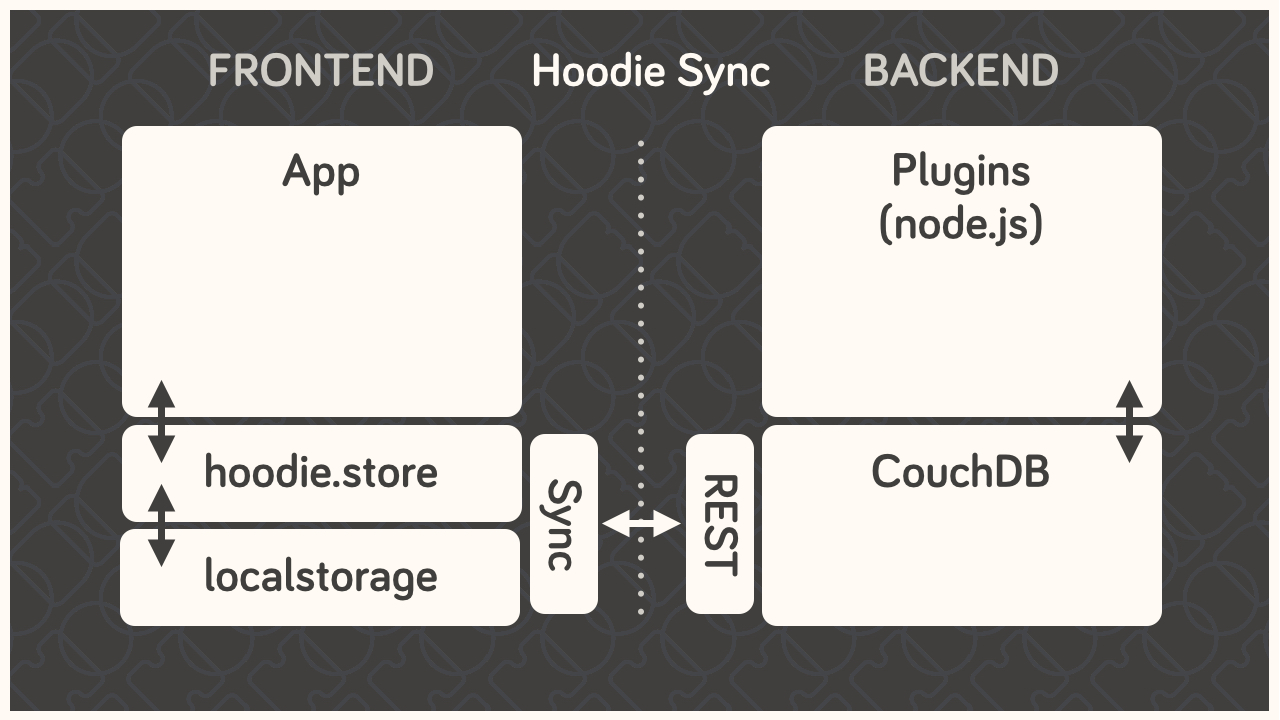
\includegraphics[width=0.8\textwidth]{hoodie}
  \grayRule
  \caption[Hoodie Architektur]{Hoodie Architektur~Quelle:~\cite{hoodie-how}}
  \label{fig:hoodie}
\end{figure}
Im Frontend--Bereicht ist die App zu sehen die über das Hoodie \gls{API} mit dem lokalen Speicher kommuniziert. Die Anwendung spricht niemals direkt mit dem Server oder der Datenbank. Für die lokale Speicherung der Daten benutzt Hoodie intern PouchDB, was wiederum IndexedDB verwendet. Durch das lokale Speichern sind die Daten auch offline verfügbar. Dann werden über eine \gls{REST} Schnittstelle mit einer CouchDB synchronisiert. CouchDB ist eine Datenbank mit der Superkraft des Synchronisierens und in Hoodie haben alle AnwenderInnen ihre eigene private CouchDB. Hinter der Datenbank befindet sich ein kleiner Server der auf die Daten in der CouchDB reagiert, die wiederum die Änderungen an den Client schickt ~\cite{hoodie-how}.
So können NutzerInnen nur auf ihre eigenen Daten zugreifen. Wenn es mehrere Geräte gibt, die mit einem Account assoziiert werden, werden die Änderungen von einem Gerät zuerst auf die serverseitige CouchDB synchronisiert, um dann von dort in die lokalen Datenbanken der anderen Geräte zu gelangen.\\
Dadurch dass das Frontend und das Backend nicht direkt miteinander sprechen, ist die Funktionalität beider Komponenten auch dann gewährleistet, wenn die Verbindung unterbrochen wird.
%
% Couch
%
\sub{\label{sec:couch}CouchDB}
Apache CouchDB\tm ist ein \gls{DBMS} das seit 2005 als freie Software entwickelt wird. Die dokumentenorientierte \gls{DB} funktioniert sowohl als einzelne Instanz, als auch im Cluster, in dem ein Datenbanksserver auf einer beliebig großen Anzahl an Servern oder \glspl{VM} ausgeführt werden kann. So kann die Datenschicht beliebig skaliert werden, um die Anforderungen vieler BenutzerInnen zu erfüllen. CouchDB verwendet das \gls{HTTP}--Protokoll und \gls{JSON} als Datenformat, weswegen es mit jeder Webfähigen Anwendung kompatibel ist. CouchDB wird über ein \gls{REST}ful \gls{HTTP} \gls{API} angesprochen. Mit den für \gls{REST}ful Services standardisierten Methoden z. B. GET, POST, PUT, DELETE können die Daten abgerufen und. manipuliert werden.\\
Das implementierte Replikationsmodell erlaubt die Synchronisation bzw. bidirektionale Replikation zu verschiedenen Geräten ist genau die Besonderheit, die CouchDB als eine Offline--Datenbank auszeichnet. Dessen Funktionsweise wird in \autoref{sec:replication} detailliert beschrieben. Dieses Protokoll ist die Grundlage für Offline First Anwendungen.
Das Replikations-API von CouchDB bietet die Möglichkeit, eine Datenbank kontinuierlich oder selbstgesteuert mit einer anderen zu synchronisieren.
So kann beispielsweise eine CouchDB-Instanz auf dem Mobiltelefon und eine auf dem Laptop bestehen und beide können sich bei bestehender Internetverbindung synchronisieren. Da so die gespeicherten Daten aus dem lokalen Speicher gelesen werden, sind ein schnelles Interface und eine geringe Latenz die positive Folge. Wenn Konflikte auftreten, beispielsweise durch gleichzeitiges Bearbeiten eines Dokuments von zwei Personen ohne Netzwerkverbindung, werden diese als solche markiert, jedoch nicht von selbst aufgelöst. So gehen keine Daten verloren und es liegt an der benutzenden Person diese zu lösen. \todo{Referenz git?}\\
CouchDB ist für Server konzipiert. Für Browser gibt es \hyperref[sub:pouch]{PouchDB} und für native iOS- und Android--\glspl{App} wurde Couchbase Lite entwickelt. Alle können Daten miteinander replizieren und verwenden das CouchDB Replikationsprotokoll~\cite{couch}.
\todo{CouchDB Replikationsmodell hier?}
%
% Pouch
%
\sub{\label{sub:pouch}PouchDB}
\todo{Was benutzt Poch wann? -- IndexedDB, Web SQL, LevelDB}
Als Ergänzung zu CouchDB kann PouchDB verwendet werden. PouchDB ist eine Open--Source--JavaScript--Datenbank, die so konzipiert wurde, dass sie im Browser läuft. PouchDB ermöglicht es Anwendungen zu erstellen, die sowohl offline als auch online funktionieren. Daten können lokal gespeichert werden, sodass alle Funktionen der Anwendung auch im Offline--Modus zur Verfügung stehen.
Daten werden unabhängig von der nächsten Anmeldung (des nächsten Onlinezugangs) zwischen \b{Clients}, CouchDB oder kompatiblen Servern synchronisiert.
PouchDB läuft auch in Node.js\footnote{JavaScript Laufzeitumgebung, steht unter \url{https://nodejs.org/en/download/} zum Download bereit} und kann als direkte Schnittstelle zu CouchDB--kompatiblen Servern verwendet werden~\cite{pouch}.